% Created by tikzDevice version 0.12.6 on 2026-03-18 00:13:14
% !TEX encoding = UTF-8 Unicode
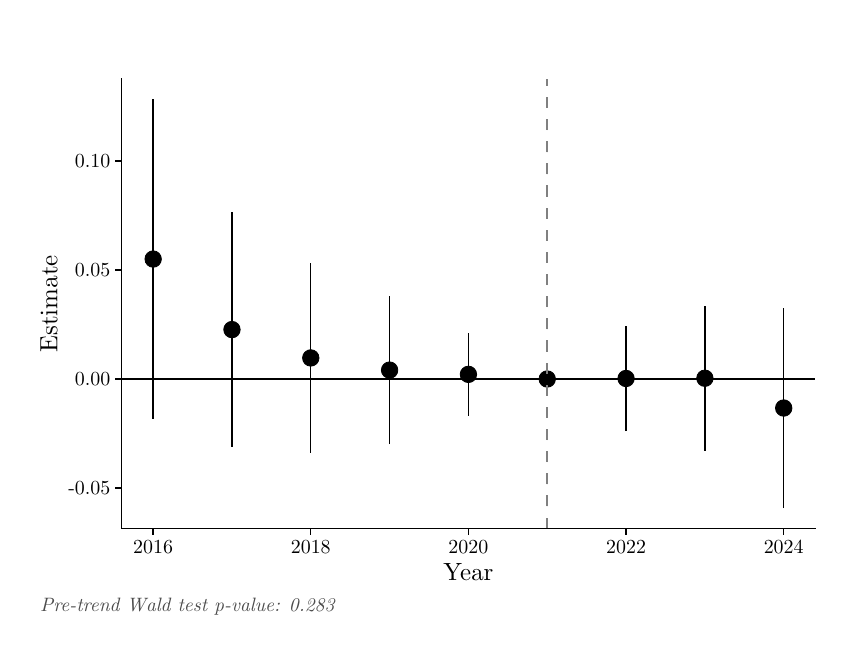
\begin{tikzpicture}[x=1pt,y=1pt]
\definecolor{fillColor}{RGB}{255,255,255}
\path[use as bounding box,fill=fillColor,fill opacity=0.00] (0,0) rectangle (289.08,216.81);
\begin{scope}
\path[clip] (  0.00,  0.00) rectangle (289.08,216.81);
\definecolor{drawColor}{RGB}{255,255,255}
\definecolor{fillColor}{RGB}{255,255,255}

\path[draw=drawColor,line width= 0.5pt,line join=round,line cap=round,fill=fillColor] (  0.00,  0.00) rectangle (289.08,216.81);
\end{scope}
\begin{scope}
\path[clip] ( 33.94, 35.79) rectangle (284.58,198.27);
\definecolor{fillColor}{RGB}{255,255,255}

\path[fill=fillColor] ( 33.94, 35.79) rectangle (284.58,198.27);
\definecolor{drawColor}{RGB}{0,0,0}

\path[draw=drawColor,line width= 0.3pt,dash pattern=on 4pt off 4pt ,line join=round] (187.74, 35.79) -- (187.74,198.27);

\path[draw=drawColor,line width= 0.3pt,line join=round] ( 33.94, 89.86) -- (284.58, 89.86);

\path[draw=drawColor,line width= 0.5pt,line join=round] ( 45.34, 75.51) -- ( 45.34,190.89);

\path[draw=drawColor,line width= 0.5pt,line join=round] ( 73.82, 65.33) -- ( 73.82,150.09);

\path[draw=drawColor,line width= 0.5pt,line join=round] (102.30, 63.26) -- (102.30,131.68);

\path[draw=drawColor,line width= 0.5pt,line join=round] (130.78, 66.36) -- (130.78,119.78);

\path[draw=drawColor,line width= 0.5pt,line join=round] (159.26, 76.64) -- (159.26,106.41);

\path[draw=drawColor,line width= 0.5pt,line join=round] (187.74, 89.86) -- (187.74, 89.86);

\path[draw=drawColor,line width= 0.5pt,line join=round] (216.22, 71.05) -- (216.22,109.02);

\path[draw=drawColor,line width= 0.5pt,line join=round] (244.71, 64.01) -- (244.71,116.26);

\path[draw=drawColor,line width= 0.5pt,line join=round] (273.19, 43.17) -- (273.19,115.57);
\definecolor{fillColor}{RGB}{0,0,0}

\path[draw=drawColor,line width= 0.3pt,line join=round,line cap=round,fill=fillColor] ( 45.34,133.20) circle (  2.97);

\path[draw=drawColor,line width= 0.3pt,line join=round,line cap=round,fill=fillColor] ( 73.82,107.71) circle (  2.97);

\path[draw=drawColor,line width= 0.3pt,line join=round,line cap=round,fill=fillColor] (102.30, 97.47) circle (  2.97);

\path[draw=drawColor,line width= 0.3pt,line join=round,line cap=round,fill=fillColor] (130.78, 93.07) circle (  2.97);

\path[draw=drawColor,line width= 0.3pt,line join=round,line cap=round,fill=fillColor] (159.26, 91.53) circle (  2.97);

\path[draw=drawColor,line width= 0.3pt,line join=round,line cap=round,fill=fillColor] (187.74, 89.86) circle (  2.97);

\path[draw=drawColor,line width= 0.3pt,line join=round,line cap=round,fill=fillColor] (216.22, 90.04) circle (  2.97);

\path[draw=drawColor,line width= 0.3pt,line join=round,line cap=round,fill=fillColor] (244.71, 90.13) circle (  2.97);

\path[draw=drawColor,line width= 0.3pt,line join=round,line cap=round,fill=fillColor] (273.19, 79.37) circle (  2.97);

\path[draw=drawColor,line width= 0.6pt,line join=round] ( 33.94, 89.86) -- (284.58, 89.86);
\definecolor{drawColor}{gray}{0.50}

\path[draw=drawColor,line width= 0.6pt,dash pattern=on 4pt off 4pt ,line join=round] (187.74, 35.79) -- (187.74,198.27);
\end{scope}
\begin{scope}
\path[clip] (  0.00,  0.00) rectangle (289.08,216.81);
\definecolor{drawColor}{RGB}{0,0,0}

\path[draw=drawColor,line width= 0.5pt,line join=round,line cap=rect] ( 33.94, 35.79) --
	( 33.94,198.27);
\end{scope}
\begin{scope}
\path[clip] (  0.00,  0.00) rectangle (289.08,216.81);
\definecolor{drawColor}{RGB}{0,0,0}

\node[text=drawColor,anchor=base east,inner sep=0pt, outer sep=0pt, scale=  0.72] at ( 29.89, 47.97) {-0.05};

\node[text=drawColor,anchor=base east,inner sep=0pt, outer sep=0pt, scale=  0.72] at ( 29.89, 87.38) {0.00};

\node[text=drawColor,anchor=base east,inner sep=0pt, outer sep=0pt, scale=  0.72] at ( 29.89,126.80) {0.05};

\node[text=drawColor,anchor=base east,inner sep=0pt, outer sep=0pt, scale=  0.72] at ( 29.89,166.21) {0.10};
\end{scope}
\begin{scope}
\path[clip] (  0.00,  0.00) rectangle (289.08,216.81);
\definecolor{drawColor}{RGB}{0,0,0}

\path[draw=drawColor,line width= 0.5pt,line join=round] ( 31.69, 50.45) --
	( 33.94, 50.45);

\path[draw=drawColor,line width= 0.5pt,line join=round] ( 31.69, 89.86) --
	( 33.94, 89.86);

\path[draw=drawColor,line width= 0.5pt,line join=round] ( 31.69,129.28) --
	( 33.94,129.28);

\path[draw=drawColor,line width= 0.5pt,line join=round] ( 31.69,168.69) --
	( 33.94,168.69);
\end{scope}
\begin{scope}
\path[clip] (  0.00,  0.00) rectangle (289.08,216.81);
\definecolor{drawColor}{RGB}{0,0,0}

\path[draw=drawColor,line width= 0.5pt,line join=round,line cap=rect] ( 33.94, 35.79) --
	(284.58, 35.79);
\end{scope}
\begin{scope}
\path[clip] (  0.00,  0.00) rectangle (289.08,216.81);
\definecolor{drawColor}{RGB}{0,0,0}

\path[draw=drawColor,line width= 0.5pt,line join=round] ( 45.34, 33.54) --
	( 45.34, 35.79);

\path[draw=drawColor,line width= 0.5pt,line join=round] (102.30, 33.54) --
	(102.30, 35.79);

\path[draw=drawColor,line width= 0.5pt,line join=round] (159.26, 33.54) --
	(159.26, 35.79);

\path[draw=drawColor,line width= 0.5pt,line join=round] (216.22, 33.54) --
	(216.22, 35.79);

\path[draw=drawColor,line width= 0.5pt,line join=round] (273.19, 33.54) --
	(273.19, 35.79);
\end{scope}
\begin{scope}
\path[clip] (  0.00,  0.00) rectangle (289.08,216.81);
\definecolor{drawColor}{RGB}{0,0,0}

\node[text=drawColor,anchor=base,inner sep=0pt, outer sep=0pt, scale=  0.72] at ( 45.34, 26.78) {2016};

\node[text=drawColor,anchor=base,inner sep=0pt, outer sep=0pt, scale=  0.72] at (102.30, 26.78) {2018};

\node[text=drawColor,anchor=base,inner sep=0pt, outer sep=0pt, scale=  0.72] at (159.26, 26.78) {2020};

\node[text=drawColor,anchor=base,inner sep=0pt, outer sep=0pt, scale=  0.72] at (216.22, 26.78) {2022};

\node[text=drawColor,anchor=base,inner sep=0pt, outer sep=0pt, scale=  0.72] at (273.19, 26.78) {2024};
\end{scope}
\begin{scope}
\path[clip] (  0.00,  0.00) rectangle (289.08,216.81);
\definecolor{drawColor}{RGB}{0,0,0}

\node[text=drawColor,anchor=base,inner sep=0pt, outer sep=0pt, scale=  0.90] at (159.26, 16.93) {Year};
\end{scope}
\begin{scope}
\path[clip] (  0.00,  0.00) rectangle (289.08,216.81);
\definecolor{drawColor}{RGB}{0,0,0}

\node[text=drawColor,rotate= 90.00,anchor=base,inner sep=0pt, outer sep=0pt, scale=  0.90] at ( 10.70,117.03) {Estimate};
\end{scope}
\begin{scope}
\path[clip] (  0.00,  0.00) rectangle (289.08,216.81);
\definecolor{drawColor}{gray}{0.30}

\node[text=drawColor,anchor=base west,inner sep=0pt, outer sep=0pt, scale=  0.70] at (  4.50,  5.86) {\itshape Pre-trend Wald test p-value: 0.283};
\end{scope}
\end{tikzpicture}
